
%6%%6%%6%%6%%6%%6%%6%%6%%6%%6%%6%%6%%6%%6%%6%%6%%6%%6%%6
%                     Validação                        %
%6%%6%%6%%6%%6%%6%%6%%6%%6%%6%%6%%6%%6%%6%%6%%6%%6%%6%%6

\chapter{Estudo de validação}

\label{chap:evaluation}

Para avaliar a estratégia que apresentamos no Capítulo \ref{chap:metrics}, conduzimos um estudo empírico a fim de analisar se as métricas que propomos são capazes de identificar as soft skills dos indivíduos que utilizam o juiz online Huxley.

Neste estudo, consideramos a relação que existe entre as soft skills e os fatores de personalidade que discutimos no Capítulo \ref{chap:concepts}. Propomos comparar se o resultado obtido através da aplicação das métricas identificam as soft skills associadas aos fatores de personalidade de um indivíduo. Para isso, coletamos as métricas que detalhamos na Seção \ref{sec:metrics} em um grupo de usuários do Huxley. Em seguida, os convidamos para responder um breve questionário a respeito de personalidade, com o objetivo de comparar os resultados. 

Para explicar o estudo de validação, apresentamos os participantes e o material na Seção \ref{sec:participantes} e Seção \ref{sec:material}, respectivamente. Na Seção \ref{sec:procedimento}, detalhamos o procedimento que seguimos durante a avaliação das métricas para identificação de soft skills. Na Seção \ref{sec:ameacas}, discutimos as principais ameaças à validade e como as contornamos.

\section{Participantes}
\label{sec:participantes}

Os participantes do estudo de validação são usuários do Huxley e estudantes matriculados nas disciplinas de Programação 1 dos cursos de Ciência da Computação e Engenharia da Computação, na Universidade Federal de Alagoas. A Tabela \ref{tab:participantes} distribui o número de participantes por semestre e curso:

\begin{table*}[ht]
\footnotesize
\caption{\small Participantes}
\addtolength{\tabcolsep}{-3.5pt}
\renewcommand{\arraystretch}{1.4} 
\centering

\begin{tabular}{|c|c|c|}
\hline
\textbf{Semestre} & \textbf{Curso} 		& 	\textbf{Número de estudantes matriculados} \\ \hline
2014.1 & Ciência da Computação 		 		& 	33 		\\ \hline
2014.1 & Engenharia da Computação 		& 	23 		\\ \hline
\multicolumn{2}{|c|}{\textbf{Total}} 	&		56 		\\ \hline
\end{tabular}

\label{tab:participantes}
\end{table*}

A disciplina de Programação 1, em ambos os cursos, tem o objetivo de capacitar o estudante em assuntos que envolvem análise e resolução de problemas, desenvolvimento de algoritmos utilizando linguagem de programação, estruturação de programas, noções de tipos e estrutura elementares de dados e conceitos de recursão \cite{cc:projeto, ec:projeto}. Atualmente, a linguagem de programação C é utilizada durante a disciplina.

Com o objetivo de estimular os estudantes, os professores incentivam a utilização do Huxley para prática e aprendizagem de programação de forma espontânea. Todos os problemas de programação contidos no sistema estão disponíveis para submissão a qualquer momento, ou seja, os alunos podem acessar o Huxley para atividades extraclasse e estabelecer seu próprio ritmo de estudos.

As aulas de Programação 1 aconteceram em um laboratório de informática. Durante as aulas, os professores utilizaram problemas do Huxley para resolvê-los como exercício. O uso do juiz online foi obrigatório apenas para atividades avaliativas, compondo parcialmente a nota de desempenho na disciplina.

No final do período de aulas, o banco de dados do Huxley guardava as interações dos usuários participantes com relação a suas atividades de programação durante a disciplina, as quais foram analisadas de acordo com as métricas para identificação de soft skills.
Nesse mesmo tempo,  
tivemos acesso presencial às turmas, para que os participantes respondessem o questionário a respeito da personalidade, de maneira que a medição das soft skills e as respostas dos questionários ocorreram em períodos de tempo muito próximos.
%, diferença de no máximo duas semanas.
Estudantes de outras turmas não foram incluídos, pois não obtivemos acesso aos mesmos dessa forma.
%O acesso presencial foi importante para que todos os participantes respondessem o questionário no mesmo período em que as soft skills foram identificadas pelas métricas. Discutiremos na Seção \ref{sec:procedimento} mais detalhes sobre a aplicação do mesmo.

\section{Material}
\label{sec:material}

O material utilizado neste estudo consiste de mais de 450 problemas de programação contidos na base de dados do Huxley. Esses problemas estão disponíveis para qualquer usuário do sistema, e portanto, para todos os participantes.

Utilizamos ainda a base de dados do Huxley para coletar as métricas, com base no histórico de participação dos usuários, considerando o período dos seis primeiros meses de uso do sistema. De forma geral, juntos os participantes enviaram 18.234 submissões para 326 problemas de programação do Huxley. Dessas submissões, 5.796 foram avaliadas como soluções corretas.

%Convidamos os participantes para responder um questionário a respeito de personalidade, chamado TIPI – Ten-Item Personality Inventory \cite{gosling:03}. Esse questionário foi proposto contendo apenas 10 itens como uma medida breve dos Cinco Fatores de personalidade, tratamos desse modelo (FFM) na Seção \ref{sec:ffm}. De acordo com os autores, o TIPI pode ser utilizado como alternativa a instrumentos longos, como o NEO PI-R, que contém 240 itens. Isso nos oferece mais espaço e tempo para focar no que está mais diretamente relacionado a nossa pesquisa, ou seja, as soft skills. Na Figura \ref{fig:tipi}, observe o questionário TIPI em sua versão original.

Também faz parte do material empregado neste estudo um questionário a respeito de personalidade chamado TIPI (Ten-Item Personality Inventory).
O TIPI foi proposto por Gosling et al. (2003)\nocite{gosling:03}
contendo apenas 10 itens como uma medida breve dos Cinco Fatores de personalidade.
Tratamos desse modelo (FFM) na Seção \ref{sec:ffm}. Para responder o TIPI, os indivíduos inquiridos utilizam uma escala Likert de 7 pontos para avaliação (entre discordo fortemente e concordo fortemente).

De acordo com os autores, o questionário TIPI pode ser utilizado como alternativa a instrumentos longos, como o NEO PI-R, que contém 240 itens. Isso nos oferece mais espaço e tempo para focar no que está mais diretamente relacionado a nossa pesquisa, ou seja, as soft skills. Na Figura \ref{fig:tipi}, observe o questionário TIPI em sua versão original, escrito no idioma Inglês.

\begin{figure}[ht]
\centering
\caption{\small Ten-Item Personality Inventory (TIPI)}
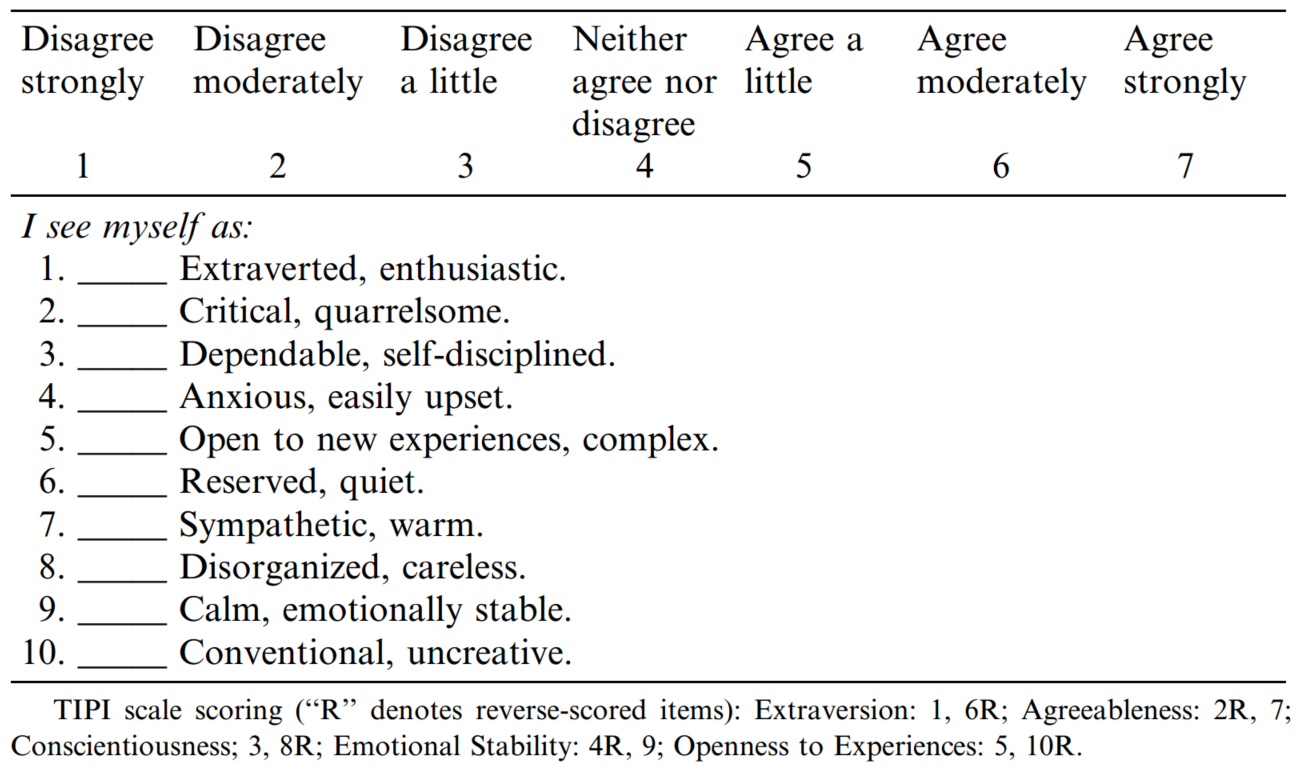
\includegraphics[width=.9\textwidth]{tipi.png}
\label{fig:tipi}
\fonte{\cite{gosling:03}}
\end{figure}

\section{Procedimento}
\label{sec:procedimento}

O procedimento do estudo de validação pode ser descrito em três passos, conforme ilustrado na Figura \ref{fig:estudo}.

No primeiro passo, aplicamos as métricas que detalhamos na Seção \ref{sec:metrics} para cada participante, utilizando a base de dados do Huxley. O período que consideramos para a coleta dos dados inicia-se na data de cadastro do usuário. A partir dessa data, analisamos a participação do mesmo, segundo a Tabela \ref{tab:dadosmetricas}, durante seis meses de uso do sistema. Esse período foi definido de acordo com o tempo do curso de Programação 1, período no qual os usuários mais utilizam o Huxley.%, que é de um semestre.

\begin{figure}[ht]
\centering
\caption{\small Procedimento do estudo de validação} 
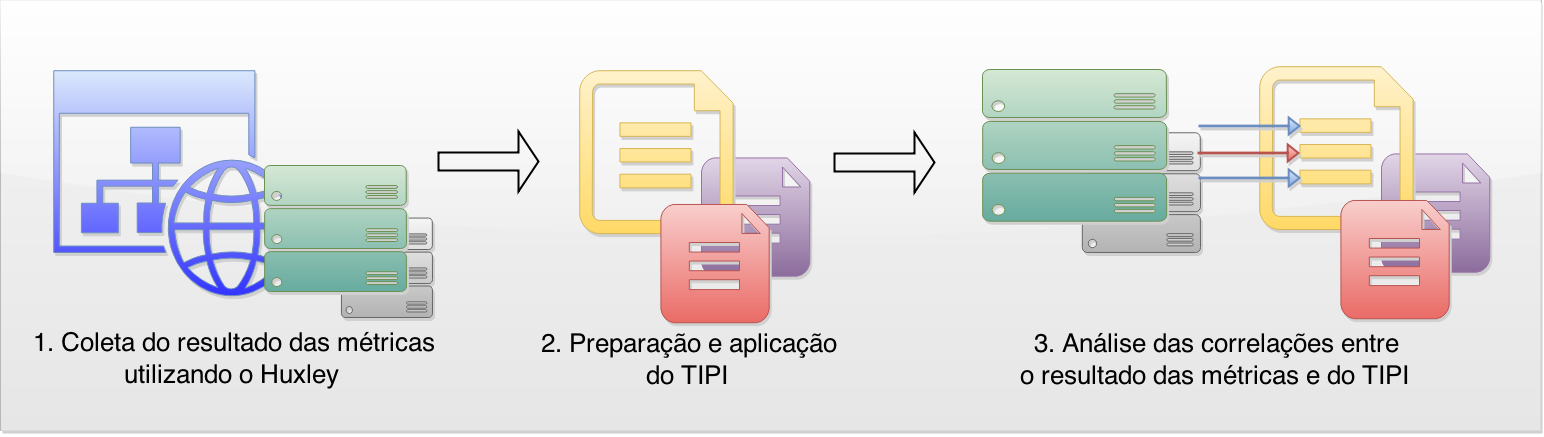
\includegraphics[width=.99\textwidth]{estudo.png}
\label{fig:estudo}
\end{figure}

Em seguida, no passo 2, preparamos o questionário TIPI para aplicá-lo ao grupo de participantes. O TIPI foi traduzido para Português buscando-se manter o significado de cada item. Apesar de alguns desses itens não estarem relacionados com as soft skills, não os removemos do questionário. Dessa forma, o apresentamos completo para avaliação dos participantes, mantendo-o o mais próximo possível de seu original para não comprometer a consistência dos itens.
%Além disso, disponibilizamos um link para acesso do TIPI em Inglês, caso o participante achasse necessário.

A fim de esclarecer o objetivo do questionário, também foram adicionadas informações contextuais aos itens. Essas informações adicionais tratam-se de frases curtas que permitem ao participante entender que suas respostas devem ser dadas de acordo com seu comportamento enquanto pratica atividades de programação. Como recomendado por John e Srivastava (1999)\nocite{john:99}, adicionar esclarecimentos ou informações contextuais em instrumentos curtos é importante para evitar problemas de mal-entendimento, como ambiguidade ou significados múltiplos.
O Apêndice \ref{ap:tipi} apresenta o instrumento que aplicamos durante este estudo de validação, nele pode-se ler os itens do TIPI e as informações contextuais que adicionamos.

O questionário TIPI foi aplicado presencialmente e individualmente para os participantes do estudo. No momento da aplicação, esclarecemos aos estudantes que suas participações não eram obrigatórias. Informamos também que suas identidades não seriam divulgadas, garantindo o anonimato das respostas, de forma que eles se sentissem à vontade para responder as questões de forma sincera.

A aplicação do TIPI ocorreu na última semana de aulas das disciplinas de Programação 1, ou seja, no mesmo período de tempo que as métricas das soft skills foram coletadas, no final do semestre. Nem todos os participantes estavam presentes, apenas 32 deles responderam o questionário. Em geral, nessa fase final da disciplina, os estudantes estão em menor número, pois muitos deixam de ir para as aulas ou mesmo desistem. Apesar de coletarmos as métricas para todos os matriculados, apenas os dados dos que responderam o questionário TIPI participam da verificação dos resultados.
%Mesmo porque, não faz sentido considerar soft skills de programador daqueles que nem sequer finalizaram a disciplina.

Então, para atingir o objetivo deste estudo, verificamos se os resultados que encontramos aplicando as métricas correspondem aos resultados do questionário, constituindo o passo 3.
Para isso, estamos considerando o coeficiente de correlação de Pearson entre as pontuações das soft skills e pontuações do teste de personalidade.
Baseamos este estudo, na relação que existe entre as soft skills e os fatores de personalidade que discutimos no Capítulo \ref{chap:concepts}.

Nossa hipótese é a seguinte: Uma métrica para identificação de soft skill pode ser validada se a mesma avalia sua respectiva soft skill em um nível que condiz com os traços de personalidade do indivíduo. Isso porque, se o indivíduo possui um determinado traço de personalidade, ele tende a possuir as soft skills relacionados a esse traço.

\section{Ameaças}
\label{sec:ameacas}

Algumas ameaças devem ser consideradas com relação a este estudo de validação, bem como precisamos discutir maneiras de contorná-las.
Inicialmente, sabemos que o fato de o questionário TIPI ser aplicado como um instrumento de auto avaliação pode levar a algum participante não o responder sinceramente. Isso pode acontecer porque alguém pode não se sentir à vontade de falar sobre si mesmo, e ainda, em nosso contexto onde os participantes são alunos, os mesmos podem ter receio de responder alguma declaração de forma negativa e dar conhecimento a seu professor de Programação.

Para lidar com esses possíveis problemas, consideramos analisar a consistência das respostas de cada participante. Para isso, calculamos as correlações dos itens do TIPI entre si. Os itens estão organizados em pares, de forma que, para cada fator do FFM existe um item positivo e um negativo. Por exemplo, o item \textit{1. Extrovertido, entusiasmado} indica o traço positivo do fator Extroversão. Já o item \textit{6. Reservado, quieto} é o traço negativo, ou inverso, indicando Introversão. Dessa forma, se um item do TIPI expressa uma declaração oposta a outro item, é preciso identificar uma correlação negativa entre os mesmos. Essa correlação deve assegurar a consistência das respostas.

Além disso, a fim de garantir que os participantes respondessem o questionário livremente, como já explicado na Seção \ref{sec:procedimento} sobre o procedimento, fizemos os estudantes cientes de que suas participações neste estudo eram opcionais e que seus dados não seriam expostos com identificação.

Outra ameaça considerada é a possibilidade de o participante não entender o questionário, ou não interpretar corretamente alguma declaração. Por esse motivo, traduzimos o questionário TIPI para o idioma Português com o cuidado de manter o instrumento o mais próximo possível de seu original. Também adicionamos informações contextuais para auxiliar os participantes a entenderem o contexto do questionário. Além de optarmos pela aplicação presencial, de forma que nos disponibilizamos a retirar qualquer dúvida no momento da coleta das respostas.

Durante as fases do estudo de validação, buscamos aplicar essas estratégias para contornar as possíveis ameaças e com a execução do mesmo fomos capazes de recolher dados suficientes para analisar os resultados desta pesquisa. A seguir, o Capítulo \ref{chap:results} vai tratar desses resultados.

